
%(BEGIN_QUESTION)
% Copyright 2010, Tony R. Kuphaldt, released under the Creative Commons Attribution License (v 1.0)
% This means you may do almost anything with this work of mine, so long as you give me proper credit

Calculate the time elapsed between the reference and echo pulses for this guided-wave radar transmitter:

$$\includegraphics[width=15.5cm]{i03685x01.eps}$$

$t$ = \underbar{\hskip 50pt} nanoseconds

\vskip 10pt

Also, write a single equation solving for this time ($t$) in terms of permittivity ($\epsilon_r$) and ullage ($x$).  Avoid compound fractions in your answer if at all possible:

\underbar{file i03685}
%(END_QUESTION)





%(BEGIN_ANSWER)

$t$ = \underbar{\bf 10.63} nanoseconds \hskip 30pt $t = {2x \sqrt{\epsilon_r} \over c}$

\vskip 10pt

5 points for numerical answer, 5 points for equation (compound-fraction version is worth 4 points).

%(END_ANSWER)





%(BEGIN_NOTES)

{\bf This question is intended for exams only and not worksheets!}.

%(END_NOTES)


